\subsubsection{summary-suGlobalManagementOfEvent}

\label{RE-use-case-suGlobalManagementOfEvent}


The goal is to manage the creation of a new crisis event including all the necessary information and to have the requested coordinators arrive on the crisis event's location.		  


\begin{usecase}
  \addheading{Use-Case Description}
  \addsingletwocolumnrow{Name}{suGlobalManagementOfEvent}
  \addsingletwocolumnrow{Scope}{system}
  \addsingletwocolumnrow{Level}{summary}
  

\addrowheading{Primary actor(s)}
\addnumberedsinglerow{}{\msrcode{actCentralCoordinator[active]}}


\addrowheading{Secondary actor(s)}
\addnumberedsinglerow{}{\msrcode{actCommunicationCompany[active]}}
\addnumberedsinglerow{}{\msrcode{actFiremenCoordinator[active]}}
\addnumberedsinglerow{}{\msrcode{actTowServiceCoordinator[active]}}

\addrowheading{Goal(s) description}
\addsinglerow{The goal is to manage the creation of a new crisis event including all the necessary information and to have the requested coordinators arrive on the crisis event's location.}

\addrowheading{Reuse}
\addnumberedsinglerow{}{\msrucname{ugCreateNewCrisisEvent [1..*]}}
\addnumberedsinglerow{}{\msrucname{ugGlobalDispatchManagement [1..*]}}

\addrowheading{Protocol condition(s)}
\addnumberedsinglerow{}{
none.}

\addrowheading{Pre-condition(s)}
\addnumberedsinglerow{}{
none.}

\addrowheading{Main post-condition(s)}
\addnumberedsinglerow{}{
a new crisis event has been created and modifications have been made by the coordinators to the system and its environment concerning a crisis event.}

\addrowheading{Main Steps}
\addalphanumberedsinglerow{}{the actor \msrcode{actCentralCoordinator} executes the \msrucname{ugCreateNewCrisisEvent} use case}
\addalphanumberedsinglerow{}{the actor \msrcode{actFiremenCoordinator} executes the \msrucname{ugGlobalDispatchManagement} use case}
\addalphanumberedsinglerow{}{the actor \msrcode{actTowServiceCoordinator} executes the \msrucname{ugGlobalDispatchManagement} use case}
\addrowheading{Steps Ordering Constraints}
\addnumberedsinglerow{}{step (a) must be executed before step (b) or step (c)}
\addnumberedsinglerow{}{step (b) XOR step (c)}

\addrowheading{Additional Information}
\addsinglerow{
none
}

\end{usecase} 


Figure \ref{fig:lu.uni.lassy.excalibur.group09.spec-RE-UCD-uc-suGlobalManagementOfEvent}
Shows the suGlobaManagementOfEvent use-case and its actors.

\begin{figure}[htbp]
\begin{center}

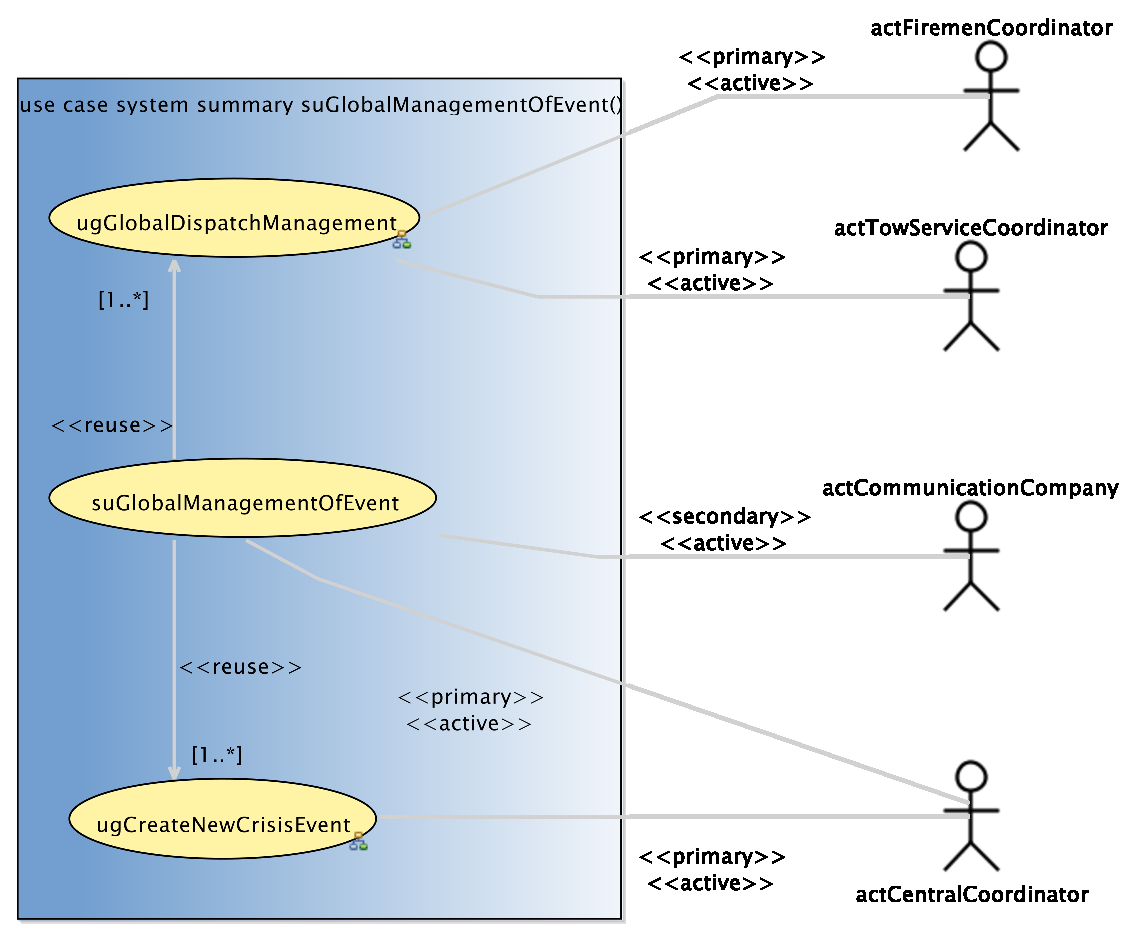
\includegraphics[
angle=0
,width=1.0\textwidth
]{./images-report-gen/usecase-model/summary/uc-suGlobalManagementOfEvent.eps}
\end{center}
\caption[lu.uni.lassy.excalibur.group09.spec Use Case Diagram: uc-suGlobalManagementOfEvent]{}
\label{fig:lu.uni.lassy.excalibur.group09.spec-RE-UCD-uc-suGlobalManagementOfEvent}
\end{figure}
\vspace{0.5cm}
